%!TEX root = ../main.tex
\chapter{Preliminaries}\label{chap:preliminaries}
\section{Probabilistic Constellation Shaping}
In this section our goal is to present the capacity limitations of the commonly used \cgls{ask} and \cgls{qam} modulation schemes. These schemes are penalized for two reasons:
\begin{enumerate}
\item They use uniform probability densities.
\item The constellation points are equidistant.
\end{enumerate}
In the following we explain the nature of these penalties.
\subsection{Introduction}
We begin with an important result from Information theory. Under a second-moment constraint, also known as power constraint, the probability distribution which maximizes the differential entropy is the Gaussian distribution, denoted with $p_G$. We thus have
\begin{align}
\label{eqn:max_entropy_scalar}
	h(X) \leq \dfrac{1}{2} \log \left(2 \pi e \sigma^2 \right)
\end{align}
where $\sigma^2 = \mathbb{E}[X^2]$, and with equality if and only if $X$ is Gaussian-distributed. More generally in the multi-dimensional case we have  
\begin{align}
\label{eqn:max_entropy_n}
	h(\underline{X}) \leq \dfrac{1}{2} \log \left((2 \pi e)^n |\textbf{Q}_{\underline{X}}| \right)
\end{align}
where we have considered a random column vector $\underline{X}$ of dimension n, mean $\mathbb{E}[\underline{X}]= \underline{m}$ and covariance matrix
\begin{align}
	\textbf{Q}_{\underline{X}}  = \mathbb{E}[(\underline{X} - \underline{m})(\underline{X} - \underline{m})^\intercal]
\end{align}
and equality in (\ref{eqn:max_entropy_n}) if only if the elements of $\underline{X}$ are jointly Gaussian.\\

\begin{figure}[ht]
\centering
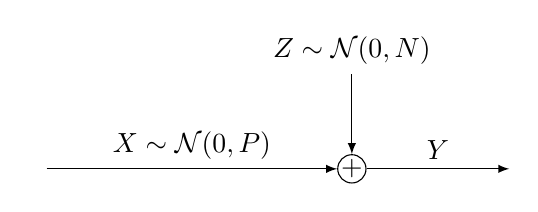
\begin{tikzpicture}
    \node(src){};
    \node[circle, draw, inner sep=0cm]at (4,0) (plus){$+$};
	
	\node at (4,1.5)(z){$Z\sim\mathcal{N}(0,N)$};

	\draw[-latex] (src) --  (plus) node[midway,above] {$X\sim\mathcal{N}(0, P)$};
	\draw[-latex] (plus) -- node[midway,above] {$Y$} (6,0);	
	
	\draw[-latex](z)--(plus);
\end{tikzpicture}
\end{figure}

Lets now consider an \cgls{awgn} channel with Gaussian input $X$, of zero mean and variance $P$; Gaussian noise $Z$, of zero mean and variance $N$; and output $Y$; i.e. $Y = X + Z$. %A visual representation of the \cgls{awgn} channel is provided in Figure \ref{}.

Furthermore, the capacity of the \cgls{awgn} is
\begin{align}
\label{eqn:awgn_cap}
	C(P) &= \max\limits_{P_X:\mathbb{E}[X^2] \leq P} \mathbb{I}(X;Y)\\
	& = \max\limits_{P_X:\mathbb{E}[X^2] \leq P}[h(Y) - h(Y \vert X)]\\
	& = \dfrac{1}{2} \log (2 \pi e (P+N)) - \dfrac{1}{2} \log (2 \pi e N)\\
	& = \dfrac{1}{2} \log \left(1 + \dfrac{P}{N} \right). 
\end{align}
We can express the mutual information
\begin{align}
\label{eqn:MI}
	\mathbb{I}(X;Y) = h(Y) - h(Y \vert X)
\end{align}
in two parts, the differential entropy of the output and the conditional differential entropy of the output given the input.
We expand the second term as
\begin{align}
	h(Y \vert X) &= h(Y - X \vert X) \\
	& = h(Z \vert X)\\
	& = h(Z) = \dfrac{1}{2} \log \left(2 \pi e \sigma^2 \right)
\end{align}
and observe that the term $h(Y \vert X)$ does not depend on how $X$ is distributed. In contrast, $h(Y)$ does depend on how $X$ is distributed by
\begin{align}
	p_Y(y) = \int_{-\infty}^{\infty} p_X(X)p_Z(y -x) \,dx = (p_X \star p_Z)(y).
\end{align}
To circumvent the fact that it is difficult to find a closed-form expression of $h(Y)$, we make use of the information divergence as
\begin{align}
\label{eqn:hy_ce}
	h(Y) \overset{\text{(a)}}{=}  h(Y_G) - \mathbb{D}(p_Y \Vert p_G)
\end{align}
where (a) arises from the fact that $\mathbb{X}(p_X \Vert p_G) = h(Y_G)$ if and only if $p_X$ has zero mean and variance P as $p_G$. (\ref{eqn:hy_ce}) is very useful as it allows us to express the differential entropy of the output in terms of the information divergence between $p_G$ and any other distribution by means of the cross entropy. 

Now we can rewrite \ref{eqn:MI} as
\begin{align}
	\mathbb{I}(X;Y) &= h(Y) - h(Y \vert X)\\
	& = h(Y) - h(Z)\\
	& = h(Y_G) - \mathbb{D}(p_Y \Vert p_G) - h(Z)\\
	& = [h(Y_G) - h(Z)] - \mathbb{D}(p_Y \Vert p_G)\\
	& = C(P/\sigma^2) - \mathbb{D}(p_Y \Vert p_G).
\label{eq:C_minus_D}
\end{align}
This last result indicates that the loss of MI when using a distribution $P_X$ different than $P_G$ is the informational divergence $\mathbb{D}(p_Y \Vert p_G)$. In other words, if the gaussian distribution is not used, the capacity penalty is characterized by $\mathbb{D}(p_Y \Vert p_G)$.\\

\subsection{Capacity Gap for Uniform Continuous Input}
\begin{figure}[ht!]
\centering
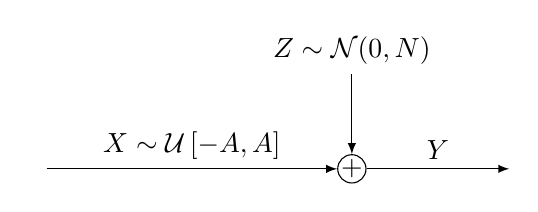
\begin{tikzpicture}
    \node(src){};
    \node[circle, draw, inner sep=0cm]at (4,0) (plus){$+$};
	
	\node at (4,1.5)(z){$Z\sim\mathcal{N}(0,N)$};

	\draw[-latex] (src) --  (plus) node[midway,above] {$X\sim\mathcal{U}\left[-A, A\right]$};
	\draw[-latex] (plus) -- node[midway,above] {$Y$} (6,0);	
	
	\draw[-latex](z)--(plus);
\end{tikzpicture}
\end{figure}
We would like now to understand how far a uniform distribution is from (\ref{eqn:max_entropy_scalar}). To do this, we will follow the approach presented in \cite{BoechererCM} to lower bound the MI. Start by defining $X_u$ as a uniformly distributed input on the interval $[-A, A]$ where A is carefully chosen so that $\mathbb{E}[{X_u}^2] = P$. The corresponding output is $Y_u$ and we proceed
\begin{align}
	\mathbb{I}(X_u;Y_u) &= C(\text{snr}) - \mathbb{D}(p_{Y_u} \Vert p_{Y_G})\\
	& \geq C(\text{snr}) - \mathbb{D}(p_{X_u} \Vert p_{X_G})\\
	& = C(\text{snr}) -[h(X_G) - h(X_u)]\\
	& = C(\text{snr}) - \dfrac{1}{2} \log_{2} \left(\dfrac{\pi e}{6}\right).
	\label{eqn:gap}
\end{align}
In Figure \ref{fig:capacity_gap} we display the derived lower bound and observe that the capacity loss, originated from the use of a uniform input density, is never more than $\dfrac{1}{2}\log_2\dfrac{\pi e}{6}$ independent of the \cgls{snr}.
\begin{figure}
	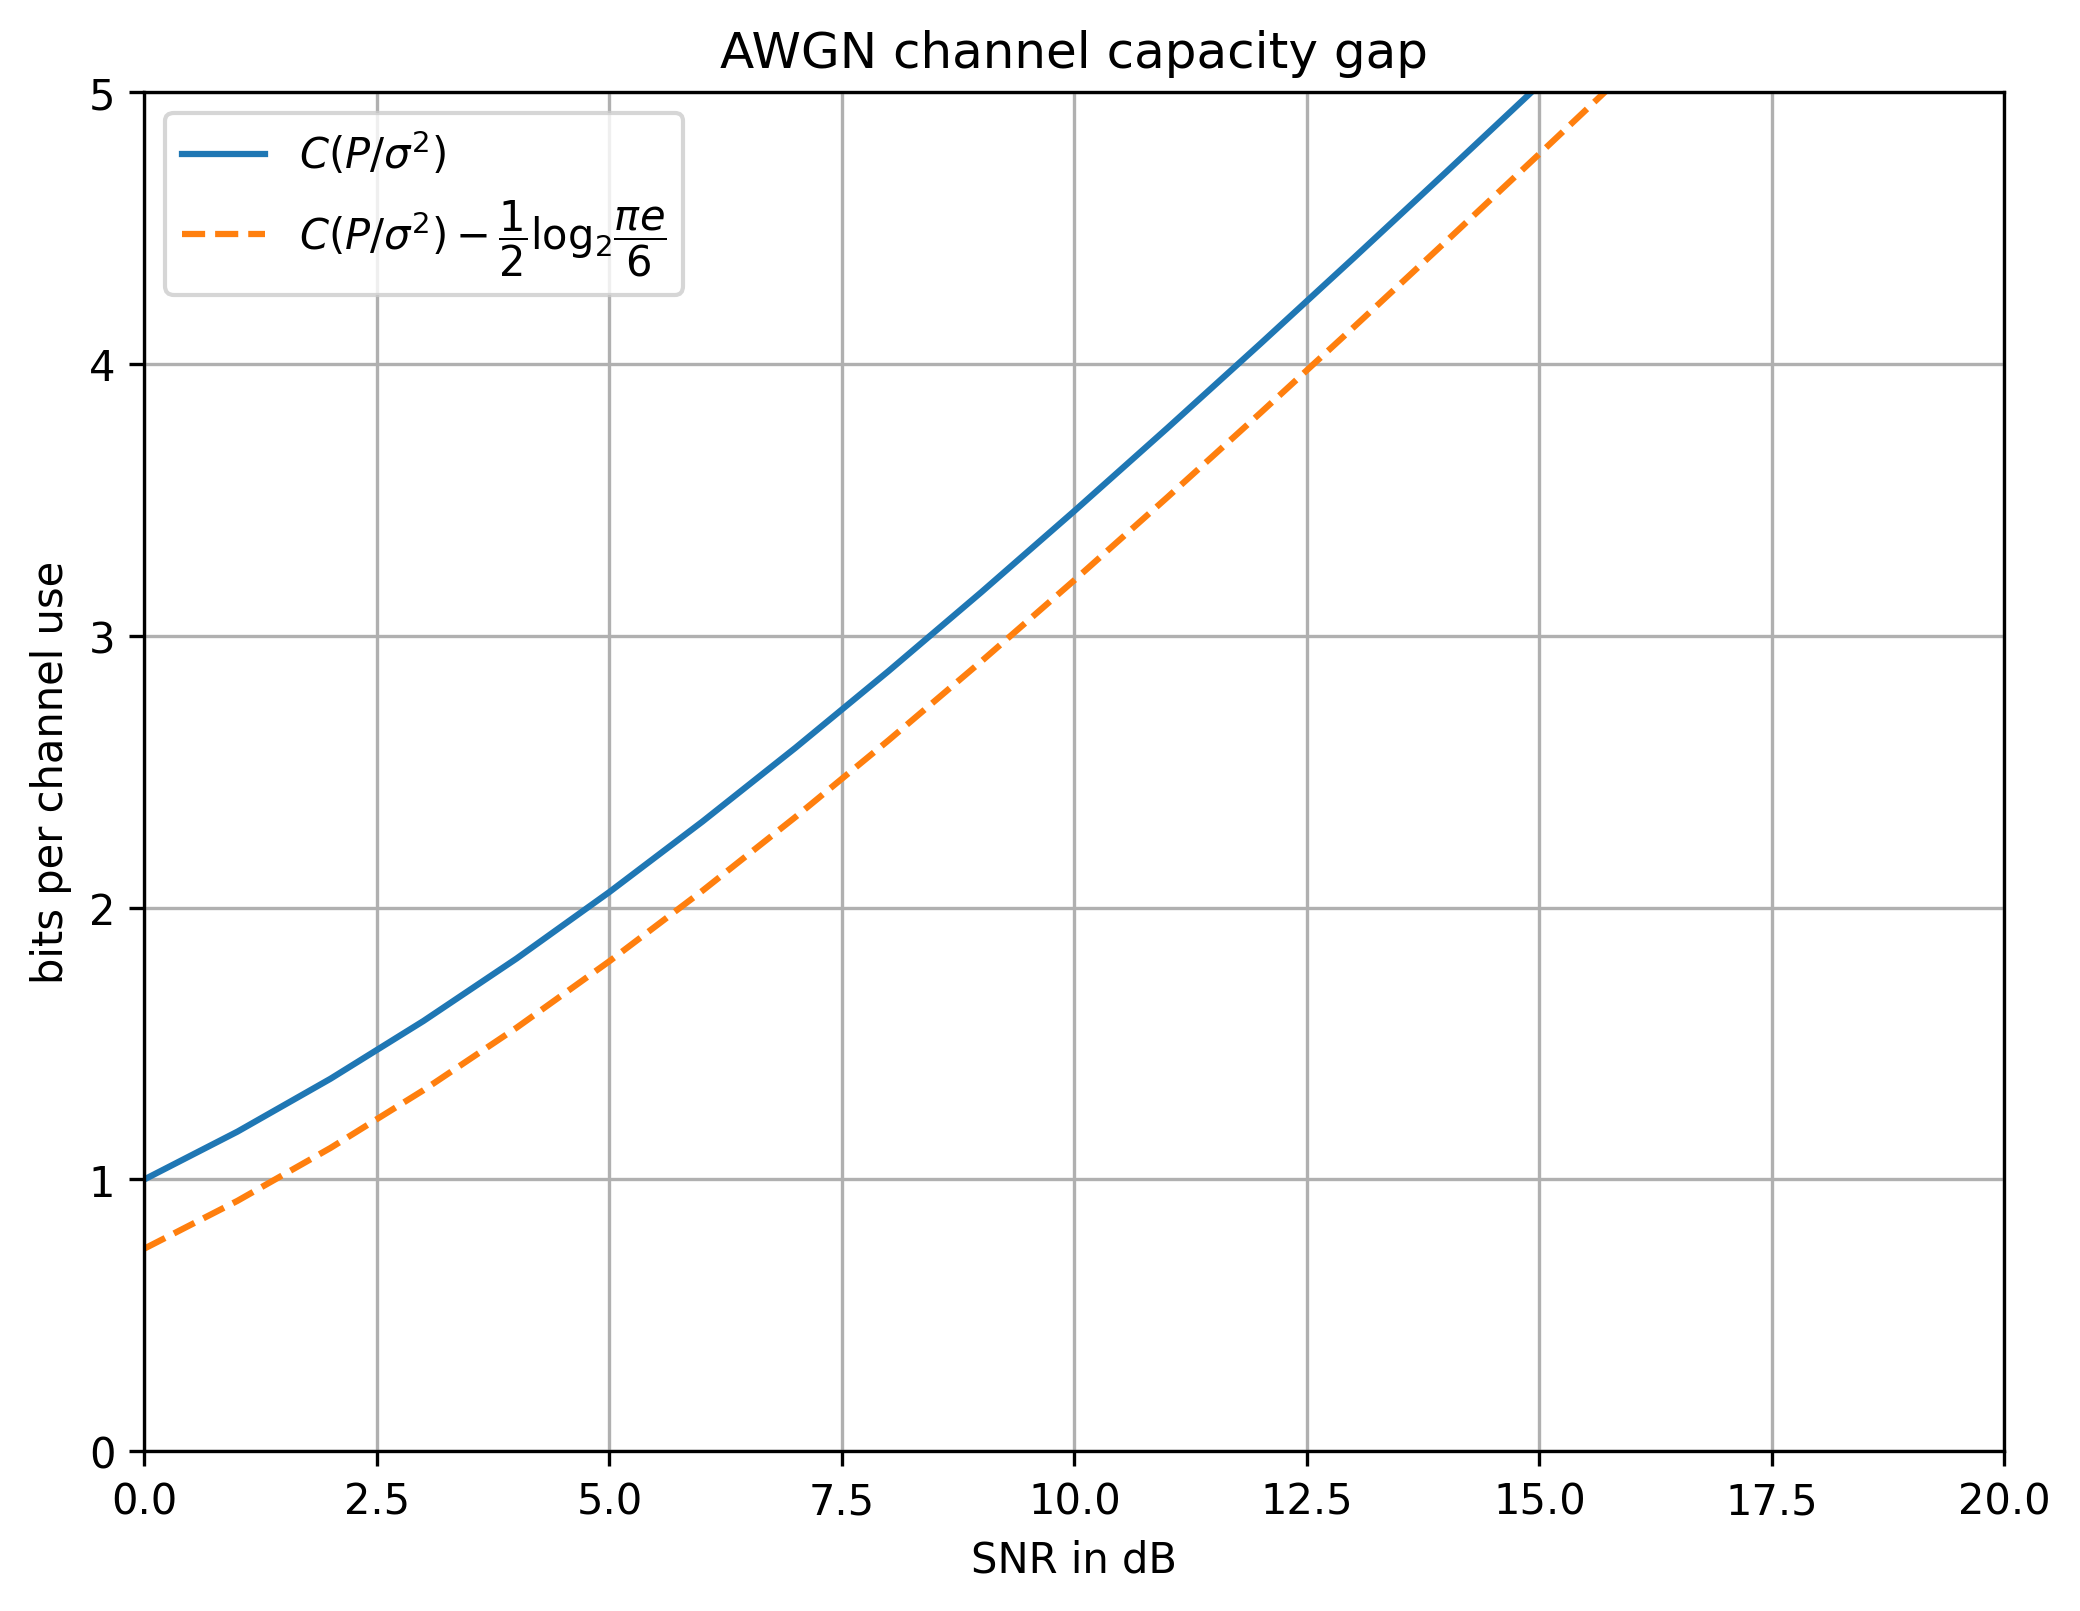
\includegraphics[width=\textwidth]{figs/capacity_gap.png}
	\caption{AWGN channel capacity gap. The orange line indicates the upper capacity bound for any uniformly distributed constellation.}
    \label{fig:capacity_gap}
\end{figure}
To show that the shaping gap is tight, it is necessary to proof an upper bound for $\mathbb{I}(X_u;Y_u)$ that approaches \ref{eqn:gap} with increasing \cgls{snr}. We refer the reader to \cite{BoechererCM}, Section 4.3, for this proof.
\subsection{Uniform Discrete Input Bound}
We now show the penalty received for the use of an equidistant M-\cgls{ask} constellation. We define the constellation points as
\begin{align}
	\mathcal{X} = \{\pm\Delta 1, \pm\Delta 3,\dots, \Delta(M-1)\},
\end{align}
where $\Delta$ is the scaling factor of the constellation, so that the channel input is $X$. If $X_M$ is uniformly distributed, the resulting power  is
\begin{align}
	P = \mathbb{E}\left[X_{M}^2\right] = \Delta^2\frac{M^2 - 1}{3}.
\end{align}
\begin{theorem}[Uniform Discrete Input Bound]
\label{th:uniform_discrete_input_bound}
The mutual information achieved by $X_M$ is lowered bounded by
\begin{align}
\mathbb{I}(X_M;Y_M) &\geq \dfrac{1}{2} \log_2 \left( \dfrac{M^2}{M^2 -1}\right) - \dfrac{1}{2} \log_2 \left[2\pi e\left( \dfrac{P}{M^2 -1}+ \dfrac{P}{1+P/\sigma^2}\right)\right]\\
& < C(\text{snr}) - \dfrac{1}{2} \log_{2} \left(\dfrac{\pi e}{6}\right) - \dfrac{1}{2} \log_2 \left[1 +\left(\dfrac{2^{C(\text{snr})}}{M}\right)^2\right]\\
& < C(\text{snr}) - \text{Penalty}(\text{Uniform dist.}) - \text{Penalty}(\text{Equidistant dist.})
\end{align}
where $\text{snr} = P/\sigma^2$.
\end{theorem}
We refer the reader to \cite{BoechererCM}, section 4.5, for the proof.
Theorem \ref{th:uniform_discrete_input_bound} shows our goal, namely that both the usage of a uniform distribution and an equidistant constellation penalizes the capacity. We can additionally compute the relation between the constellation size, $M$, and $C(\text{snr})$ so that the resulting \cgls{mi} is within a constant gap of capacity. To make this result even more attractive, we increase the constraint for the gap to match the order of the distribution loss (0.255 bits). We obtain
\begin{align}
	- \dfrac{1}{2} \log_2 \left[1 +\left(\dfrac{2^{C(\text{snr})}}{M}\right)^2\right] \leq - \dfrac{\log_2 e}{2} \left(\dfrac{2^{C(\text{snr})}}{M}\right)^2 = \dfrac{1}{4}\\
	\Leftrightarrow M = 2^{C(\text{snr}) + \tfrac{1}{2}+\tfrac{1}{2} \log_2 \log_2 e}
\end{align}
by using $\log_e(x)\leq (1-x)$. So if 
\begin{align}
	\log_2 M \approx C(\text{snr}) +0.77,
\end{align}
then the mutual information is within 0.5 bit of capacity.

% Write about Maxwel-Boltxman distributions...
\subsection{Capacity-achieving distributions}
We now address the question of finding the discrete probability distribution which maximizes the capacity. Such distribution should be free of the $ \dfrac{1}{2} \log_{2} \left(\dfrac{\pi e}{6}\right)$ penalty. We use again an \cgls{ask} constellation with M signal points ( in practice, M is a power of 2) given by 
\begin{align}
	\mathcal{X} = \{\pm 1, \pm 3,\dots, (M-1)\}.
\end{align}

Let $X$ be a random variable with distribution $P_X$ over $\mathcal{X}$. As before, we scale $X$ by a $\Delta > 0$ and the resulting input/output relation for an \cgls{awgn} channel becomes
\begin{align}
	Y = \Delta X + Z
\end{align}

In consequence, the \cgls{mi} of the channel input and output is 
\begin{align}
	\mathbb{I}(\Delta X; Y) &= \mathbb{I}(\Delta X; \Delta X + Z)\\
	&= \mathbb{I}(\Delta X; \Delta X + Z)
\end{align}

where the second equality follows because $(\Delta X)$ is a deterministic function of $X$ and vice-versa. Under an input average power constraint $P$, the scaling $\Delta$ and the distribution $P_X$ must be chosen to satisfy
\begin{align}
	\mathbb{E}[(\Delta X)^2] \leq P.
\end{align}

Formally, our optimization problem is the following

\begin{align}
	C(P/\sigma^2) &= \max\limits_{\Delta, P_X :\mathbb{E}[(\Delta X)^2] \leq P} \mathbb{I}(X;\Delta X+Z).
\end{align}

Maximizing the mutual information $\mathbb{I}(X;\Delta X+Z)$ both over the scaling of the constellation points and the input distribution requires a relatively high amount of power. Instead, as shown in \cite{BoechererCM}, section 5.3, we will use a suboptimal input distribution which follows from maximizing the input entropy.

We expand the mutual information as
\begin{align}
	\mathbb{I}(X,\Delta X+Z) &= \mathbb{H}(X) - \mathbb{H}(X| \Delta X+Z)
\end{align}
and fixing $\Delta$, we select the input distribution $P_{X_\Delta}$ that maximizes the input entropy under our power constraint, i.e., we choose
\begin{align}
	P_{X_\Delta} &= \argmax\limits_{P_X:\mathbb{E}[(\Delta X)^2] \leq P} \mathbb{H}(X).
\end{align}
Without the discrete constraint, the solution would be a Gaussian distribution. For this reason we explore sampled Gaussian distributions, also known as \cgls{mb} distributions. For each $\mathcal{X} = \{\pm1, \pm 3,\dots, (M-1)\}$, define
\begin{align}
	P_{X_v}(x_i) &= A_{\nu}e^{-\nu{x_i}^2},\text{  } A_{\nu} = \dfrac{1}{\sum\limits_{i=1}^{M}e^{-\nu{x_i}^2}} 
\end{align}

We now show that $P_{X_\Delta}$ is given by
\begin{align}
P_{X_\Delta}(x_i) = P_{X_\nu}(x_i) \text{ with } \nu : \mathbb{E}[(\Delta X_{\nu})^2] = P
\end{align}

\begin{proof}
Consider the finite set $\mathcal{X} = {x_1, x_2, \dots , x_n}$ . Let $f$ be a function that
assigns to each $x_i \in \mathcal{X}$ a positive cost $f(x_i) > 0$. Define the \cgls{mb} distribution
\begin{align}
	P_{X_v}(x_i) &= A_{\nu}e^{-\nu f(x_i)},\text{  } A_{\nu} = \dfrac{1}{\sum\limits_{i=1}^{M}e^{-\nu f(x_i)}} 
\end{align}	
Let $P_X$ be some distribution on $\mathcal{X}$ with $ \mathbb{E}[f(X)] = P $. Choose $\nu : \mathbb{E}[f(X_{\nu})] = P$
\begin{align}
	0 &\leq \mathbb{D}(P_X \Vert P_{X_{\nu}})\\
	&= \sum\limits_{x \in \text{Support}(P_{X_{\nu}})} P_X \log(\dfrac{P_X(x)}{P_{X_{\nu}}(x)}) \\
	&= -\mathbb{H}(X) - \sum\limits_{x \in \text{Support}(P_{X_{\nu}})} P_X(x) \log(P_{X_{\nu}}(x)) \\
	&\overset{\text{(*)}}{=} -\mathbb{H}(X) - \sum\limits_{x \in \text{Support}(P_{X_{\nu}})} P_{X_{\nu}}(x) \log(P_{X_{\nu}}(x)) \\
	&= -\mathbb{H}(X) + \mathbb{H}(X_{\nu}) \\
	\mathbb{H}(X) &\leq \mathbb{H}(X_{\nu})
\end{align}
where the (*) marked step follows since both distributions produce the same moments for $log(P_{X_{\nu}}(x))$.
\end{proof}


	
\section{Autoencoders}
\subsection{Introduction}
In this section we present the basics of autoencoders in the context of \cgls{dl} and communication systems, which was pioneered in \cite{O'Shea}. The idea behind an autoencoder is to transmit a particular representation of the input data so that at the output, it can be reconstructed with minimal error. This means that the desired representations must be robust with respect to the channel impairments (i.e. noise, fading, distortion, etc.). To find such representations and the corresponding mappings $\textbf{x}$ to $\textbf{y}$ we train deep \cglspl{nn}. Because \cglspl{nn} are universal function approximators \cite{HORNIK1989359}, this technique is particularly interesting for training over channels without a mathematically tractable model.

\subsection{Feed-Forward Neural Networks}
\cGlspl{ffnn} are structures capable of transforming the input vector $\bold{v_0} = (v_{0,1} \dots v_{0,M})$ into an output vector $\bold{v_k} = (v_{K,1} \dots v_{K,n})$, i.e., $\bold{v_K}=f_{\text{NN}}(\bold{v_0})$. This transformation is accomplished by composing functions, which in turn are computed by layers. Using matrix notation we can express the output of each layer as
\begin{align}
	\vb{v_k} = g_{\text{NL},k}(\vb{W}_k\vb{v}_{k-1}+\vb{b}_k), \qquad k = 1, \dots, K,
\end{align}

where k indicates the layer index, and $g_{\text{NL},k}(\cdot)$ is a nonlinear function applied between layers. Indeed, without the nonlinear function the \cgls{ffnn} lacks the expressive power required to approximate any function \cite{HORNIK1989359}.

\tikzset{
    neuron/.style={
		circle,
		draw=black,
		minimum size=0.4cm,
		fill=blue,
	},	
    neuron dark/.style={
		circle,
		draw=black,
		minimum size=0.4cm,
		fill=TUMBlueDark,
	},	
	neuron missing/.style={
		draw=none, 
		fill=white,
		scale=1.0,
		text height=0.3cm,
		execute at begin node=\color{black}$\vdots$
	},
	label/.style = {draw=none, fill=none, rectangle, minimum height=1em, minimum width=1em},
	blockrx/.style = {draw, fill=white, rectangle, minimum height=1.5em, minimum width=6.25em},
	blocktx/.style = {draw, fill=white, rectangle, minimum height=1.5em, minimum width=13em},
	block/.style = {draw, fill=white, rectangle, minimum height=2em, minimum width=10em,rounded corners},
	blockthesis/.style = {draw, fill=gray!20, rectangle, minimum height=1.5em, minimum width=40em,rounded corners},
	block1/.style = {draw, fill=white, rectangle, minimum height=1.5em, minimum width=1.5em,rounded corners},
	tmp/.style  = {coordinate}, 
	sum/.style= {draw, fill=white, circle, node distance=1cm},
	mul/.style= {draw=none, fill=white, circle, node distance=1cm},
	input/.style = {coordinate},
	output/.style= {coordinate},
	pinstyle/.style = {pin edge={to-,thin,black}
	}
}

\begin{figure}[h]
    \centering
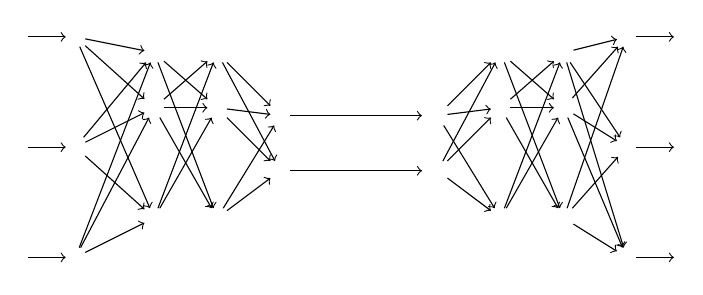
\begin{tikzpicture}
	%encoder
	\foreach \m [count=\y] in {1,missing,3,missing,5}
	\node [neuron/.try, neuron \m/.try] (input1-\m) at (0,2-\y*0.7) {};
	
	\foreach \m [count=\y] in {1,2,missing,4}
	\node [neuron/.try, neuron \m/.try ] (hidden1-\m) at (1,1.8-\y*0.7) {};
	
	\foreach \m [count=\y] in {1,2,missing,4}
	\node [neuron/.try, neuron \m/.try ] (hidden2-\m) at (1.8,1.8-\y*0.7) {};
	
	\foreach \m [count=\y] in {1,2}
	\node [neuron/.try, neuron \m/.try ] (output1-\m) at (2.6,1-\y*0.7) {};
	
	\foreach \i in {1,3}
	\draw [<-] (input1-\i) -- ++(-0.6,0);
	
	\foreach \l [count=\i] in {1,2}
	\draw [->] (output1-\i) -- ++(1.8,0);
%	node [above, midway] {$y_\i$};
	
	
	\draw [<-] (input1-5) -- ++(-0.6,0);

	%mesh1
	\foreach \i in {1,3,5} 
	\foreach \j in {1,2,4}
	\draw [->] (input1-\i) -- (hidden1-\j);
	
	\foreach \i in {1,2,4}
	\foreach \j in {2}
	\draw [->] (hidden1-\i) -- (hidden2-\j);
	
	\draw [->] (hidden1-2) -- (hidden2-1); 
	\draw [->] (hidden1-4) -- (hidden2-1); 
	
	\draw [->] (hidden1-1) -- (hidden2-4); 
	\draw [->] (hidden1-2) -- (hidden2-4); 
	
	\foreach \i in {1,2,4}
	\foreach \j in {1,2}
	\draw [->] (hidden2-\i) -- (output1-\j);
	
	%decoder
	\foreach \m [count=\y] in {1,2}
	\node [neuron/.try, neuron \m/.try ] (input2-\m) at (4.6,1-\y*0.7) {};
	
	\foreach \m [count=\y] in {1,2,missing,4}
	\node [neuron/.try, neuron \m/.try ] (hidden3-\m) at (5.4,1.8-\y*0.7) {};
	
	\foreach \m [count=\y] in {1,2,missing,4}
	\node [neuron/.try, neuron \m/.try ] (hidden4-\m) at (6.2,1.8-\y*0.7) {};
	
	\foreach \m [count=\y] in {1,missing,3,missing,5}
	\node [neuron/.try, neuron \m/.try] (output2-\m) at (7,2-\y*0.7) {};
	
	%outputs
	\foreach \i in {1,3,5}
	\draw [->] (output2-\i) -- ++(0.6,0);
	
	%mesh2
	\foreach \i in {1,2} 
	\foreach \j in {1,2,4}
	\draw [->] (input2-\i) -- (hidden3-\j);
	
	\foreach \i in {1,2,4}
	\foreach \j in {2}
	\draw [->] (hidden3-\i) -- (hidden4-\j);
	
	\draw [->] (hidden3-2) -- (hidden4-1); 
	\draw [->] (hidden3-4) -- (hidden4-1); 
	
	\draw [->] (hidden3-1) -- (hidden4-4); 
	\draw [->] (hidden3-2) -- (hidden4-4); 
	
	\foreach \i in {1,2,4}
	\foreach \j in {1,3,5}
	\draw [->] (hidden4-\i) -- (output2-\j);
	
	
	
	
\end{tikzpicture}    
\end{figure}

\subsection{Autoencoders}

\subsection{Stochastic Gradient Descent}
To find fitting sets of parameters \textbf{$\theta$}, the most used algorithm is \cgls{sgd} which starts with a random set of initial values and then updates \textbf{$\theta$} with each iteration as
\begin{align}
	\theta_{new} = \theta_{old} + \epsilon \pdv{\theta_{old}} L(\theta_{old})
\end{align}

One particular requirement for using \cgls{sgd} to train the autoencoders is that the loss gradient needs to be backpropagated
all the way through receiver and channel to the transmitter. Otherwise, the transmitter parameters cannot be updated. This in turn means, that channel and receiver must be available as differentiable functions during training.

We can now set up the problem which we would like to address in this work. Namely, to train a deep \cgls{nn}-based autoencoder system to find a parametric distribution $p_{\theta}(s)$. By maximizing the \cgls{mi} during training, the output distribution must satisfy \ref{eq:C_minus_D}, and thus, approach the channel capacity.